\textbf{El número de medallas de oro ganadas por México.}\vspace{.3cm}

\begin{center}
	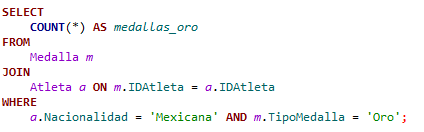
\includegraphics[width=1.05\textwidth]{resources/consulta6.png}
\end{center} 

\textbf{Explicación:} \\
En esta consulta, seleccionamos la tabla Medalla y la enlazamos con la tabla Atleta mediante un join usando IDAtleta para relacionar medallas con los atletas. Luego, aplicamos un filtro con where para incluir solo los atletas de nacionalidad mexicana y medallas de tipo oro. Finalmente, usamos count(*) para contar las filas que cumplen estas condiciones, obteniendo el total de medallas de oro ganadas por atletas mexicanos.
\vspace{.3cm}

\textbf{Resultado:}
\begin{center}
	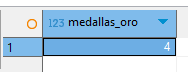
\includegraphics[width=1.05\textwidth]{resources/resultados/r6.png}
\end{center} 